% $Id: template.tex 11 2007-04-03 22:25:53Z jpeltier $

\documentclass{vgtc}                          % final (conference style)
%\documentclass[review]{vgtc}                 % review
%\documentclass[widereview]{vgtc}             % wide-spaced review
%\documentclass[preprint]{vgtc}               % preprint
%\documentclass[electronic]{vgtc}             % electronic version

%% Uncomment one of the lines above depending on where your paper is
%% in the conference process. ``review'' and ``widereview'' are for review
%% submission, ``preprint'' is for pre-publication, and the final version
%% doesn't use a specific qualifier. Further, ``electronic'' includes
%% hyperreferences for more convenient online viewing.

%% Please use one of the ``review'' options in combination with the
%% assigned online id (see below) ONLY if your paper uses a double blind
%% review process. Some conferences, like IEEE Vis and InfoVis, have NOT
%% in the past.

%% Figures should be in CMYK or Grey scale format, otherwise, colour 
%% shifting may occur during the printing process.

%% These few lines make a distinction between latex and pdflatex calls and they
%% bring in essential packages for graphics and font handling.
%% Note that due to the \DeclareGraphicsExtensions{} call it is no longer necessary
%% to provide the the path and extension of a graphics file:
%% \includegraphics{diamondrule} is completely sufficient.
%%
\ifpdf%                                % if we use pdflatex
  \pdfoutput=1\relax                   % create PDFs from pdfLaTeX
  \pdfcompresslevel=9                  % PDF Compression
  \pdfoptionpdfminorversion=7          % create PDF 1.7
  \ExecuteOptions{pdftex}
  \usepackage{graphicx}                % allow us to embed graphics files
  \DeclareGraphicsExtensions{.pdf,.png,.jpg,.jpeg} % for pdflatex we expect .pdf, .png, or .jpg files
\else%                                 % else we use pure latex
  \ExecuteOptions{dvips}
  \usepackage{graphicx}                % allow us to embed graphics files
  \DeclareGraphicsExtensions{.eps}     % for pure latex we expect eps files
\fi%

%% it is recomended to use ``\autoref{sec:bla}'' instead of ``Fig.~\ref{sec:bla}''
\graphicspath{{figures/}{pictures/}{images/}{./}} % where to search for the images

\usepackage{microtype}                 % use micro-typography (slightly more compact, better to read)
\PassOptionsToPackage{warn}{textcomp}  % to address font issues with \textrightarrow
\usepackage{textcomp}                  % use better special symbols
\usepackage{mathptmx}                  % use matching math font
\usepackage{times}                     % we use Times as the main font
\renewcommand*\ttdefault{txtt}         % a nicer typewriter font
\usepackage{cite}                      % needed to automatically sort the references
\usepackage{tabu}                      % only used for the table example
\usepackage{booktabs}                  % only used for the table example
%% We encourage the use of mathptmx for consistent usage of times font
%% throughout the proceedings. However, if you encounter conflicts
%% with other math-related packages, you may want to disable it.


%% If you are submitting a paper to a conference for review with a double
%% blind reviewing process, please replace the value ``0'' below with your
%% OnlineID. Otherwise, you may safely leave it at ``0''.
\onlineid{0}

%% declare the category of your paper, only shown in review mode
\vgtccategory{Research}

%% allow for this line if you want the electronic option to work properly
\vgtcinsertpkg

%% In preprint mode you may define your own headline.
%\preprinttext{To appear in an IEEE VGTC sponsored conference.}

%% Paper title.

\title{Value-Suppressing Uncertainty Maps}

%% This is how authors are specified in the conference style

%% Author and Affiliation (single author).
%%\author{Roy G. Biv\thanks{e-mail: roy.g.biv@aol.com}}
%%\affiliation{\scriptsize Allied Widgets Research}

%% Author and Affiliation (multiple authors with single affiliations).
%%\author{Roy G. Biv\thanks{e-mail: roy.g.biv@aol.com} %
%%\and Ed Grimley\thanks{e-mail:ed.grimley@aol.com} %
%%\and Martha Stewart\thanks{e-mail:martha.stewart@marthastewart.com}}
%%\affiliation{\scriptsize Martha Stewart Enterprises \\ Microsoft Research}

%% Author and Affiliation (multiple authors with multiple affiliations)
\author{Michael Correll\\ %
        \scriptsize University of Washington %
\and Dominik Moritz\\ %
     \scriptsize University of Washington %
\and Jeffrey Heer\\ %
     \scriptsize University of Washington}
 
%Figure list:
% Vsum vs. traditional 2D heatmap vs. juxtaposed maps
% Chart of color bins w/r/t CIELAB threshold, with iconic maps at intervals
% Process figure
% Real examples with different color maps




\newcommand{\teaserFig}{
  \teaser{
		\centering
		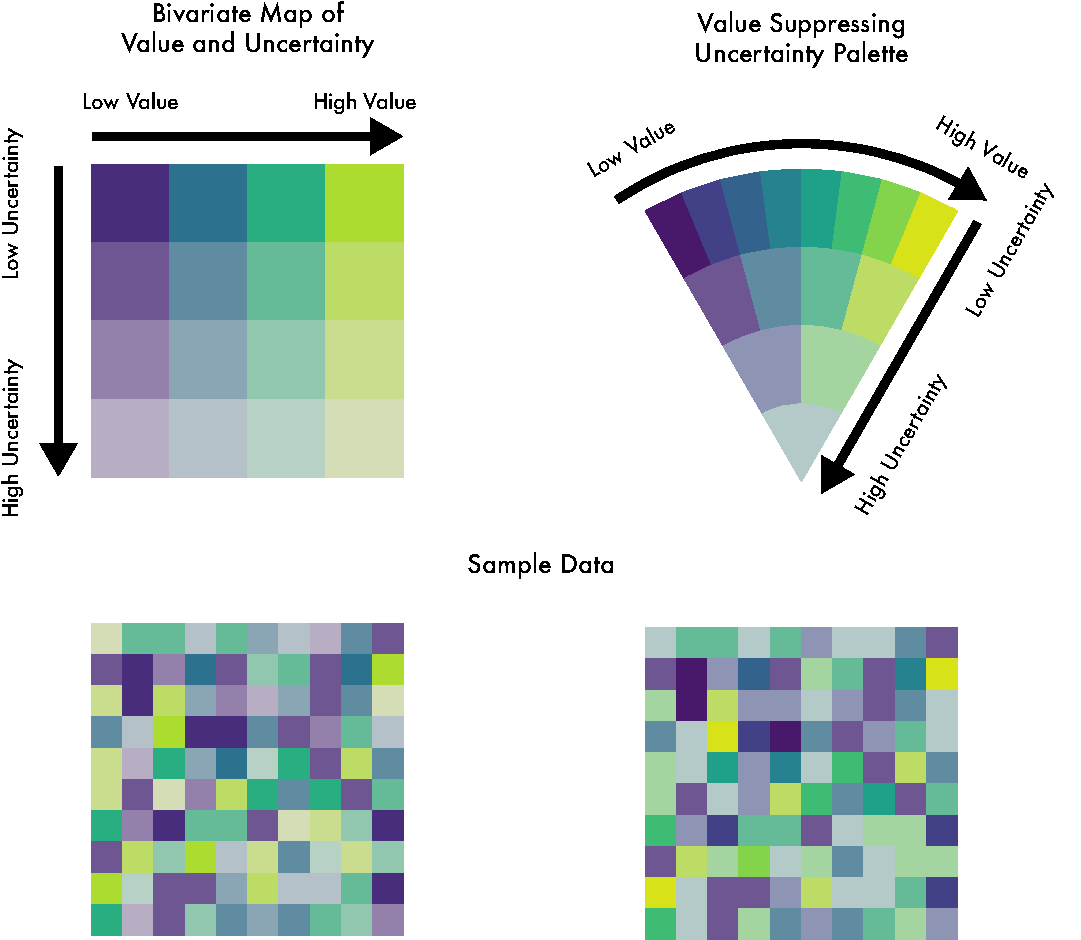
\includegraphics[width=0.9\textwidth]{example.pdf}
		\caption{Lookit! Lookit!}
		\label{fig:teaser}
	}
}

\newcommand{\exampleFig}{
\begin{figure}
	\centering
	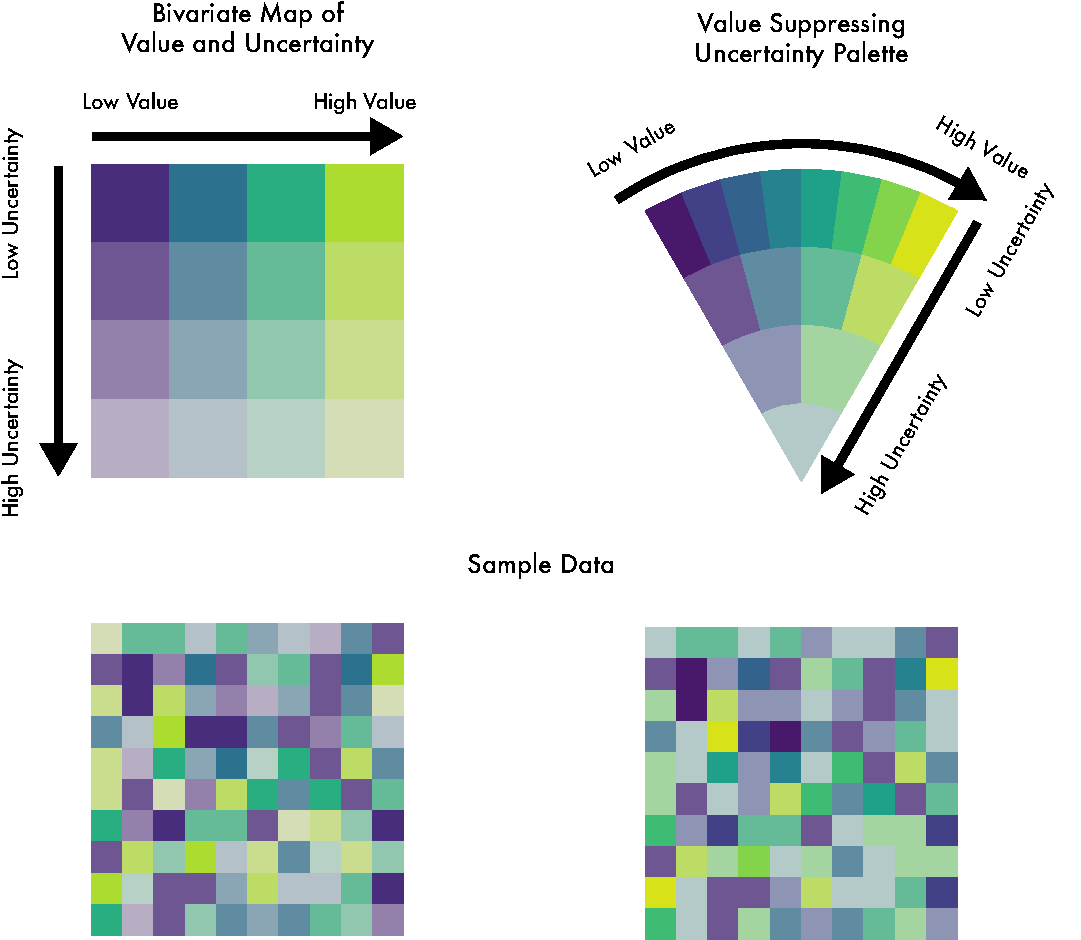
\includegraphics[width=0.9\columnwidth]{example.pdf}
	\caption{A comparison between a standard bivariate map and a VSUM. Both use the same visual channels to encode value (position along the Viridis color map) and uncertainty (lightness and saturation), and have an equal standard of perceptual discriminability (at least 18 units of distance in CIELAB color space between colors). However, highly uncertain values result in colors that are very close together in the bivariate case, meaning the full bivariate map is only 9 bins under these constraints--- a 4x4 map would result in colors that are perceptually too close together. By contrast, the VSUM intentionally reduces bins when uncertainty is high, eventually aliasing all highly uncertain values to the same color. This decision affords more distinct colors in other regions of the map, and so an increase in overall bins to 15. The resulting map suppresses the value of uncertain data, but increases the discriminability of highly certain data.}
	\label{fig:example}
\end{figure}

}

%\teaserFig
%% A teaser figure can be included as follows, but is not recommended since
%% the space is now taken up by a full width abstract.
%\teaser{
%  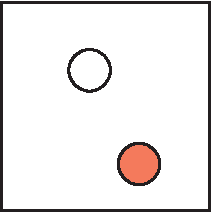
\includegraphics[width=1.5in]{sample.eps}
%  \caption{Lookit! Lookit!}
%}

%% Abstract section.
\abstract{
	
	% uncertainty-aware decisions.
	% refrain from making a decision
	% integrate uncertainty with the display
	% value-suppressing encodings
	% provide greater visual discriminability for values with high certainty, but alias together uncertain values
	% ran a study
	% results indicate X
	
	Uncertainty information is a vital part of many datasets, and should be accurately conveyed to the analyst.
	Directly integrating uncertainty information with data requires that designers construct bivariate maps that encode value and uncertainty simultaneously. The design of such bivariate maps can be difficult, and the impact of different choices of encodings on decision-making under uncertainty understudied.
    In this paper, we present a category of bivariate maps for uncertainty, ``value-suppressing uncertainty maps,'' (VSUMS). As opposed to traditional bivariate maps, VSUMS make the informed decision to alias together values when uncertainty is high, in order to afford greater discriminability when uncertainty is low. That is, certain data is intrinsically easier to visually disambiguate than uncertain data. 
    We present several examples of these maps, as well as a crowd-sourced evaluation showing X. We conclude that Y.
	
	%However, in thematic maps, strong visual variables such as position and hue are already reserved to encode location and value. 
	
	%Remaining visual variables with semiotic connection to uncertainty, such as transparency and saturation, are comparatively more difficult to discriminate, and can interfere with color discrimination.
	

	
	%Uncertainty, when it is directly encoded at all, is often visualized using visual variables with lower discriminability, or relegated to tooltips or separate charts.
 
	
} % end of abstract

%% ACM Computing Classification System (CCS). 
%% See <http://www.acm.org/class/1998/> for details.
%% The ``\CCScat'' command takes four arguments.

\keywords{Uncertainty Visualization, Color Perception, Thematic Maps, Semiotics.}

%\CCScatlist{ 
%  \CCScat{K.6.1}{Management of Computing and Information Systems}%
%{Project and People Management}{Life Cycle};
%  \CCScat{K.7.m}{The Computing Profession}{Miscellaneous}{Ethics}
%}

%% Copyright space is enabled by default as required by guidelines.
%% It is disabled by the 'review' option or via the following command:
% \nocopyrightspace

%%%%%%%%%%%%%%%%%%%%%%%%%%%%%%%%%%%%%%%%%%%%%%%%%%%%%%%%%%%%%%%%
%%%%%%%%%%%%%%%%%%%%%% START OF THE PAPER %%%%%%%%%%%%%%%%%%%%%%
%%%%%%%%%%%%%%%%%%%%%%%%%%%%%%%%%%%%%%%%%%%%%%%%%%%%%%%%%%%%%%%%%

\begin{document}

%% The ``\maketitle'' command must be the first command after the
%% ``\begin{document}'' command. It prepares and prints the title block.

%% the only exception to this rule is the \firstsection command
\firstsection{Introduction}

\maketitle

%% \section{Introduction} %for journal use above \firstsection{..} instead


% What this section needs to do:
% Uncertainty is important!
% What do we mean by ``well-integrated'' uncertainty?
% Scope down to thematic maps
% Juxtapose/superimpost distinction?
% Position bivariate maps (tacitly or explicitly) as state of the art
% Teaser image showing what we mean

Uncertainty is an inescapable component of collecting, presenting, and using data. A common goal in the communication of uncertainty is promoting \textbf{uncertainty-aware decisions}--- that is, the audience should be aware of the risks and rewards of certain decisions, modulate their confidence in their conclusions, and perhaps refrain from making a decision at all if there is too much uncertainty. A way that designers can contribute to this goal is by ensuring that uncertainty information is \textbf{well-integrated} with the rest of the data. That is, it should be difficult to discount or ignore the uncertainty in a dataset. A designer of a visualization could instantiate this principle through the simultaneous presentation of uncertainty and value. This simultaneous presentation necessitates the construction of a bivariate map--- a relation, in terms of visual variables, between a 2-tuple $(value$,$uncertainty)$ and a set of marks.

In this paper, we present \textbf{Value-Suppressing Uncertainty Maps} (VSUMs) for integrating data and uncertainty information in thematic maps. VSUMs intentionally alias together data values with high uncertainty, affording greater discriminability as certainty increases. Rather than a square bivariate map, with unique outputs for each relevant combination of data and uncertainty, VSUMs can be thought of as arcs: as uncertainty increases, values are mapped to smaller and smaller sets of outputs, culminating in a singularity where all inputs are mapped to an identical, highly uncertain mark regardless of their data value. Figure X shows an example of a VSUM, compared to a more traditional bivariate map. In this work, we describe the motivations behind the use of VSUMs, examples of their utility for decision-making under uncertainty, and validate VSUMs in a crowd-sourced experiment.
 
\section{Related Works}

% What this section needs to do:
% State of the art in uncertainty vis, with heavy emphasis on MacEachren & co. 
% Bivariate maps are hard!
% Binning colormaps is de rigueur
% The variables we'd want to use for uncertainty (like value or alpha or size) mess with color discriminability

\subsection{Visual Variables for Representing Uncertainty}

MacEachren et al. \cite{maceachren2012visual} evaluate a number of visual variables for representing uncertainty. 
\subsection{Interactions Between Visual Variables}

\section{Value-Suppressing Uncertainty Maps}


\subsection{Design}


\subsection{Examples}

\section{Evaluation}

%Show:
% 1) Juxtaposition makes people ignore/underweight uncertainty (even when they don't screw up the search task)
% 2) VSUMs make people, surprise surprise, bad at distinguishing highly uncertain values
% 3) But, they make uncertainty better-integrated
%    i) lower weights on uncertain values in decision-making
%    ii) a priori better discrimination

\subsection{Methods}

%conditions:
% 1) juxtaposed d map, u map
% 2) binned d/u map as per a priori jnds
% 3) vsm
% 4) continuous d/u map?

\subsubsection{Participants}
\subsection{Results}

\section{Discussion}
\subsection{Limitations and Future Work}
% When should you use these things?

\section{Conclusion}


%% if specified like this the section will be committed in review mode
\acknowledgments{
Omitted for review.}

%\bibliographystyle{abbrv}
\bibliographystyle{abbrv-doi}
%\bibliographystyle{abbrv-doi-narrow}
%\bibliographystyle{abbrv-doi-hyperref}
%\bibliographystyle{abbrv-doi-hyperref-narrow}

\bibliography{template}
\end{document}
